\documentclass[tikz,border=5pt]{standalone}
\usepackage{pgfplots}
\pgfplotsset{compat=1.18}
\definecolor{corba}{HTML}{365FB3}
\definecolor{punt}{HTML}{B91C1C}
\begin{document}
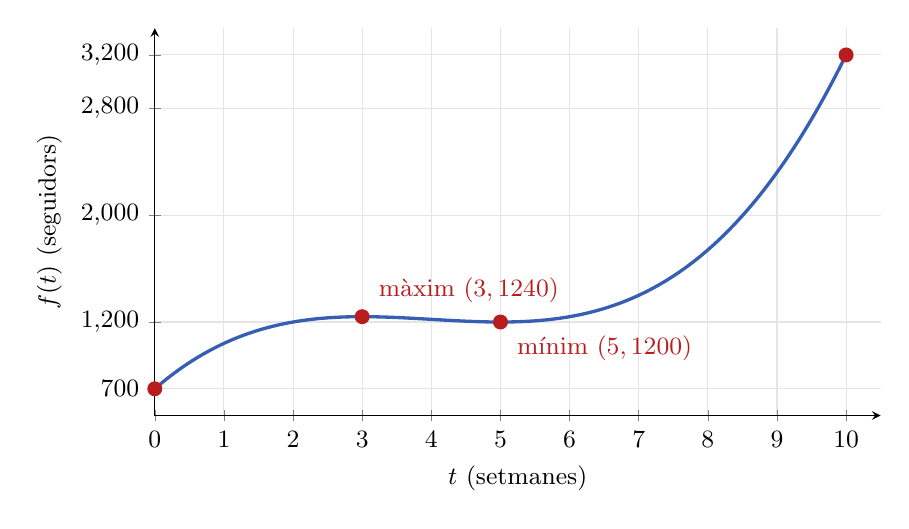
\begin{tikzpicture}
\begin{axis}[
  width=10.8cm,height=6.5cm,axis lines=left,
  xmin=0,xmax=10.5,ymin=500,ymax=3400,
  xlabel={$t$ (setmanes)},ylabel={$f(t)$ (seguidors)},
  xtick={0,1,...,10},ytick={700,1200,2000,2800,3200},
  grid=major,grid style={black!10},tick label style={font=\small},label style={font=\small},clip=false]
  \addplot[corba,very thick,domain=0:10,samples=160]{10*x^3-120*x^2+450*x+700};
  \addplot[only marks,mark=*,mark size=2.5pt,punt] coordinates {(0,700) (3,1240) (5,1200) (10,3200)};
  \node[anchor=south west,font=\small,text=punt] at (axis cs:3.1,1270) {màxim $(3,1240)$};
  \node[anchor=north west,font=\small,text=punt] at (axis cs:5.1,1170) {mínim $(5,1200)$};
\end{axis}
\end{tikzpicture}
\end{document}
